\pdfoutput=1

\documentclass[aps,prd,reprint,twocolumn,showpacs,nofootinbib,superscriptaddress,floatfix]{revtex4-1}

\usepackage{amsmath,amssymb,amstext}
\usepackage[usenames,svgnames]{xcolor}
\usepackage{hyperref,graphicx}
\usepackage{subfigure}

\hypersetup{
    colorlinks=true,
    urlcolor=SteelBlue,
    linkcolor=red,
    citecolor=blue,
}

\renewcommand{\vec}[1]{\mathbf{#1}}

\begin{document}
\title{Power spectrum and particle production\\ in galileon bouncing cosmologies}

\author{David A. Dobre}%
\email{ddobre@sfu.ca}
\affiliation{Department of Physics, Simon Fraser University,\\
8888 University Drive, Burnaby, British Columbia V5A 1S6, Canada}

\author{Andrei V. Frolov}%
\email{frolov@sfu.ca}
\affiliation{Department of Physics, Simon Fraser University,\\
8888 University Drive, Burnaby, British Columbia V5A 1S6, Canada}

\author{Jos\'{e} T. G\'{a}lvez Ghersi}%
\email{joseg@sfu.ca}
\affiliation{Department of Physics, Simon Fraser University,\\
8888 University Drive, Burnaby, British Columbia V5A 1S6, Canada}
\affiliation{Perimeter Institute for Theoretical Physics,\\
31 Caroline Street North, Waterloo, Ontario, N2L 2Y5, Canada}

\author{Alexander Vikman}%
\email{vikman@fzu.cz}
\affiliation{Institute of Physics, the Academy of Sciences of the Czech Republic,\\
Na Slovance 2, 182 21 Prague 8, Czech Republic}
\date{\today}


\begin{abstract}
In this paper, we study the main features of the scalar and tensor power spectrum of primordial fluctuations during the classically stable bouncing phase recently proposed by Ijjas and Steinhardt in Ref.~\cite{Ijjas:2016tpn}. Following the suggested background history, we evaluated the tensor and scalar spectra during the bouncing phase characterized by the violation of null (and strong) energy condition. We found that the change of the speed of sound is the cause of the dominance of the tensor power spectrum over the scalar part through most of the bounce. Moreover, we observe that none of the spectra evaluated across the bouncing phase is scale invariant. In addition to this, we present our results for particle production by showing the evolution of the occupation number of scalar fluctuations through the bounce.    
\end{abstract}

\maketitle


\section{Introduction}
Bouncing cosmologies are typically studied as effective field manifestations of many high energy theories of grand unification with extended symmetry, as shown in Refs.~\cite{Ashtekar:2006rx, Poplawski:2011jz}. Moreover, the production of healthy bouncing trajectories is an important accomplishment in order to produce a sensible expansion history free of singularities. A satisfactory non-singular bounce might not require from a complete description of the theory in the ultraviolet limit -- including Quantum Gravity -- while remaining coherent with the observed stages of homogeneity and isotropy seen in Cosmic Microwave Background (CMB). It is possible to find recent progress in the approach described in Refs.~\cite{Ijjas:2016tpn, Ijjas:2016vtq}, wherein the expansion history and the running of the kinetic couplings are used as inputs to describe the full dynamics of a cubic galileon. A valuable feature of this approach is that it is exactly the inverse when compared to other methods in which a field with a non-canonical kinetic term is used as a source (for example, in Refs.~\cite{Deffayet:2010qz, Easson:2011zy}) of the bouncing expansion history.  

The study of scalar and tensor perturbations is remarked as important across the existing literature: it adds additional constraints to the notions of a stable bouncing trajectory by avoiding all forms of instabilities such as $c_s^2<0$, tachyonic and gradient. Nevertheless, the dynamical properties of these fluctuations are not fully explored. This might be due to the cumbersome time dependence of the second-order expanded action, or because of the need of expensive computational power to resolve at higher frequencies. In this paper, we compute the numerical evolution of the scalar and tensor modes by implementing a simplified version of the separation technique described in Ref.~\cite{Ghersi:2016gee}, where each of the equations of motion of each mode is separated in two parts: one equation -- with a reduced oscillation frequency -- evolves the amplitude and another first-order equation evaluates the phase. After this separation, the numerical treatment of the system not only permits to visualize the power spectrum of curvature scalar and tensor fluctuations at a given instant of time, but all across the bouncing phase with sufficient resolution in Fourier domain. Furthermore, the dynamical evaluation of the spectra throughout the bounce is relevant since the (de-)accelerating background has a continuous effect on the perturbations. A visible effect of this acceleration is the dynamical production of particles, which can also be studied as the background evolves and will also be reflected in the particular features of the spectra.              

The plan of this paper is as follows, in section \ref{secII}, we review the features of the bouncing model explored in Ref.~\cite{Ijjas:2016tpn} and the suggested bouncing trajectory. We will study the forbidden regions of phase space for the cubic galileon, where the scalar perturbations are unstable. In addition to this, we will also find the location of the bouncing trajectories in phase space. In section \ref{secIII}, we describe the the action, equations of motion and initial conditions required to find the spectrum of scalar and tensor fluctuations. It is widely known that the choice of initial conditions is not unique, our choice was a state of instantaneous minimal energy previous to the bouncing stage in order to have properly defined initial conditions at all wavelengths. We also review the standard definition of occupancy number as stated in Ref.~\cite{Barnaby:2010ke}. In section \ref{secIV}, we show our results for the power spectra of primordial scalar and tensor fluctuations. We present two major results: (I) the power spectra are not scale invariant and (II) the scalar spectrum only dominates over the tensor by the end of the bouncing phase. In this section, we exhibit our results for scalar and tensor particle creation and its effects in the spectra. Finally, we discuss and conclude.      

\section{Background}\label{secII}

In this section, we will review the main properties of the background for bouncing scenario proposed in Ref.~\cite{Ijjas:2016tpn} as a preliminary step. The dynamics of the background is required to describe the time evolution of tensor and scalar fluctuations. In this case, the bounce is sourced by a cubic galileon:
\begin{eqnarray}
&S=\displaystyle{\int d^4x\sqrt{-g}\bigg[\frac{1}{2}M_{\mathrm{Pl}}^2R-\frac{1}{2}k(\phi)\partial_\mu\phi\partial^\mu\phi-V(\phi)}\label{cg-action}\\
&+\displaystyle{\frac{1}{4}M_{\mathrm{Pl}}^{-4}q(\phi)\left(\partial_\mu\phi\partial^\mu\phi\right)^2+\frac{1}{2}M_{\mathrm{Pl}}^{-3}b(\phi)\Box\phi~\partial_\mu\phi\partial^\mu\phi\bigg]}.\nonumber
\end{eqnarray}  
Where $k(\phi)$, $q(\phi)$ and $b(\phi)$ are dimensionless kinetic field-dependent couplings. Scalar field theories with non-canonical kinetic terms have been used to describe the behavior of an imperfect fluid, as described in Ref.~\cite{Deffayet:2010qz}. The equations of motion for the system are obtained after varying with respect to $g_{\mu\nu}$ and $\phi$. The Friedmann equations are obtained after varying with respect to $g_{\mu\nu}$, in units of $M_{\mathrm{Pl}}\equiv1$ these are given by
\begin{eqnarray}
&\rho = 3H^2 = \frac{k\dot{\phi}^2}{2}+\frac{1}{4}(3q-2b')\dot{\phi}^4+3Hb\dot{\phi}^3+V(\phi),\label{Hsquared}\\
&\rho+P = -2\dot{H} = k\dot{\phi}^2+(q-b')\dot{\phi}^4+3Hb\dot{\phi}^3-b\ddot{\phi}\dot{\phi}^2.\label{Hdot}
\end{eqnarray}
In the same way, the equation of motion of $\phi$ is given by
\begin{eqnarray*}
&\left(k+(3q-2b')\dot{\phi}^2+6Hb\dot{\phi}^2+\frac{3}{2}b^2\dot{\phi}^4\right)\ddot{\phi} =\\
&-\frac{1}{2}k'\dot{\phi}^2-\frac{1}{4}(3q'-2b'')\dot{\phi}^4-\frac{3}{4}b\left(q\dot{\phi}^4+4V\right)\dot{\phi}^2\\
&-3H\left(k+q\dot{\phi}^2+\frac{3}{2}b^2\dot{\phi}^4\right)\dot{\phi}-V',
\end{eqnarray*}
where we can notice that this is still a second-order differential equation in time. After setting $b(\phi)\equiv 1$ and defining the auxiliary function $\gamma\equiv H-\dot{\phi}^3/3$, we can invert \eqref{Hsquared} and \eqref{Hdot} in order to find the values of the couplings $k(\phi)$ and $q(\phi)$ that will be consistent with a fixed expansion history $H(t)$ and a given $\gamma(t)$   
\begin{eqnarray}
&k(t) = -2\left(3H^2-2V+2\dot{H}+\dot{\gamma}+3H\gamma\right)/\dot{\phi}^2,\nonumber\\
&q(t) = \frac{4}{3}\left(2\dot{H}+\dot{\gamma}+9H\gamma-3V\right)/\dot{\phi}^4.\nonumber
\end{eqnarray}

\begin{figure}
\begin{center}
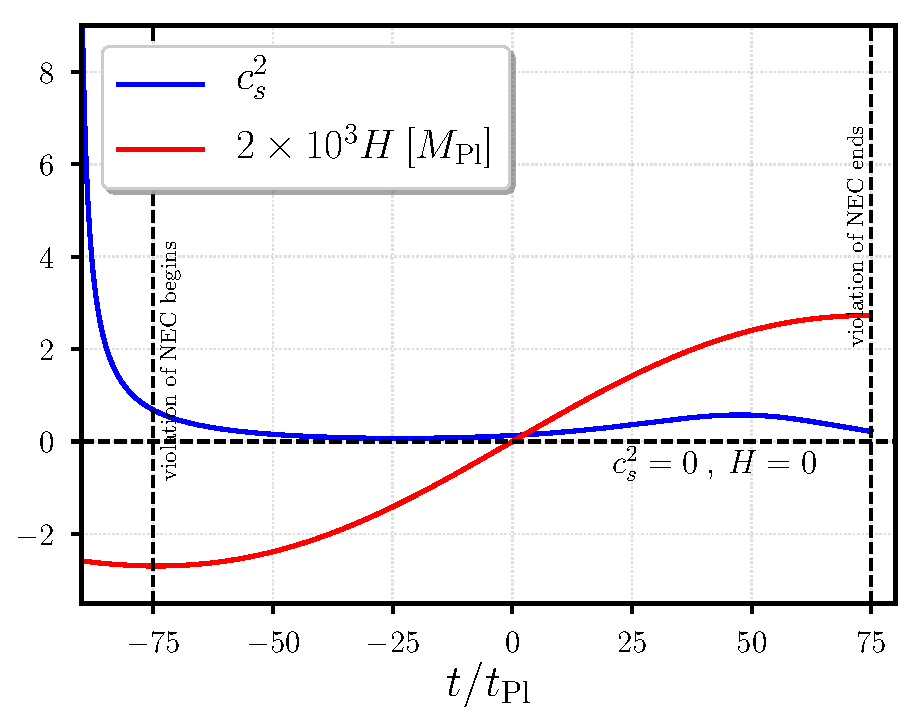
\includegraphics[width=0.45\textwidth]{full_background.pdf}
\caption{Evolution of the Hubble scale $H(t)$, $\gamma(t)$ and the speed of sound as a function of time. $\gamma(t)$ and $H(t)$ were rescaled to fit in the same plot.}
\label{fig:full_back}
\end{center}
\end{figure}

This is the essence of the so-called inverse method. Notice that in this way the evolution of $\phi$ is also fixed, and hence the complete dynamics of the background. The viability of any specific choice of an expansion history and $\gamma(t)$ still needs to be studied in phase space in the same way as in Ref.~\cite{Easson:2011zy}. In particular, we will explore the case in which $H(t)$ and $\gamma(t)$ are in the form
\begin{eqnarray}
&H(t) = H_0t e^{-F(t-t^*)^2},\label{hubblet}\\
&\gamma(t) = \gamma_0e^{3\Theta t}+H(t),\label{gammat}
\end{eqnarray}
which coincides with the choice made in Ref.~\cite{Ijjas:2016tpn} with $H_0=3\times 10^{-5}M_{\mathrm{Pl}}^2$, $\gamma_0=-0.0044M_{\mathrm{Pl}}$, $t^*=0.5M_{\mathrm{Pl}}^{-1}$, $F=7\times 10^{-5}M_{\mathrm{Pl}}^2$ and $\Theta=4.6\times10^{-6}M_{\mathrm{Pl}}$ selected as constants. In Fig.~\ref{fig:full_back}, we observe the evolution of the expressions in \eqref{hubblet} and \eqref{gammat} as a function of time. Here we also include the speed of sound ($c_s^2$) as an additional parameter which only depends on the background variables, which will be defined in full detail in the next section. As an additional comment, we do not observe any divergencies of $\gamma$ in the interval we selected for the evaluation of these functions. In Fig.~\ref{fig:NEC_SEC_violation}, we represent the intervals where the null (NEC) and strong energy conditions (SEC) are violated. We found that the violation of NEC occurs between $t_{\mathrm{NEC}}\in[-74M_{\mathrm{Pl}}^{-1};75M_{\mathrm{Pl}}^{-1}]$, while the SEC breaks in  $t_{\mathrm{SEC}}\in[-78M_{\mathrm{Pl}}^{-1};79M_{\mathrm{Pl}}^{-1}]$.

\begin{figure}
\begin{center}
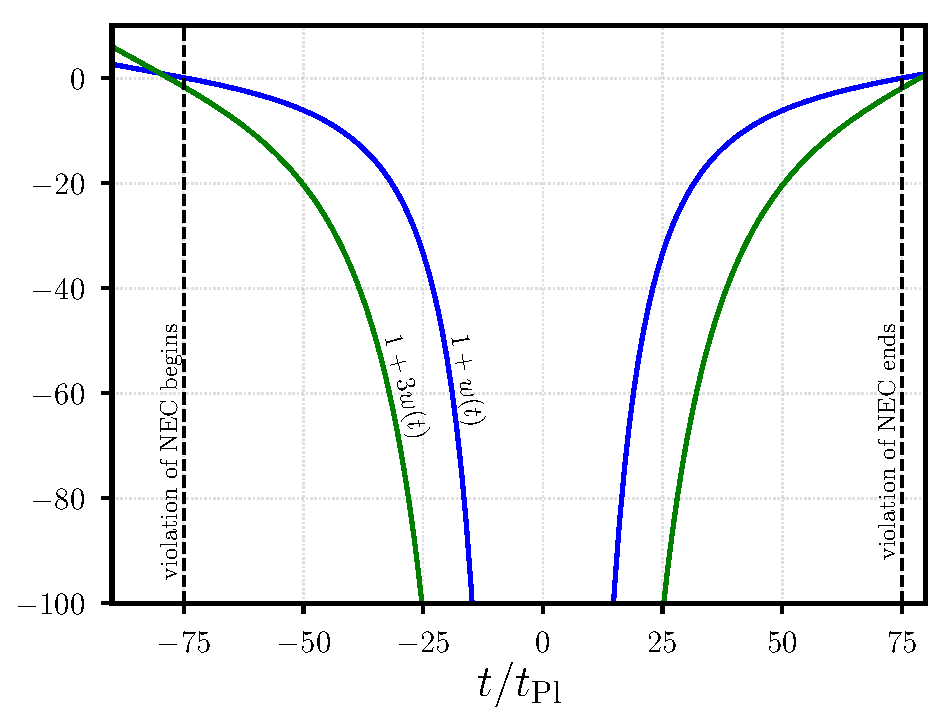
\includegraphics[width=0.45\textwidth]{NEC_SEC.pdf}
\caption{Evaluation of the null (NEC) and strong (SEC) energy conditions. Both quantities ($1+w(t)$ and $1+3w(t)$) diverge at the bounce.}
\label{fig:NEC_SEC_violation}
\end{center}
\end{figure}

In the case we study, we represented $H(t)$ and $\gamma(t)$ in a slightly expanded time interval $t\in[-90M_{\mathrm{Pl}}^{-1};75M_{\mathrm{Pl}}^{-1}]$, which now includes a regime where the speed of sound is now allowed to have superluminal values. This fact will not represent a severe problem in the evaluation of perturbations. However, we must proceed with caution at $t\geq 100M_{\mathrm{Pl}}^{-1}$ since during that period $c_s^2<0$. Such a feature should not be seen as intrinsic issue of the model since the background equations in \eqref{cg-action} does not consider any additional form of matter apart from the imperfect fluid sourced by the cubic galileon. Nevertheless, as we will see in the next section, we must avoid this regime since ghost instabilities will appear for the case of scalar curvature perturbations.      

\section{Scalar and tensor fluctuations}\label{secIII}
\section{Power spectrum of scalar and tensor fluctuations}\label{secIV}

%%%%%%%%%%%%%%%%%%%%%%%%%%%%%%%%%%%%%%%%%%%%%%%%%%%%%%%%%%%%%%%%
\begin{thebibliography}{99}

\bibitem{Ijjas:2016tpn} 
  A.~Ijjas and P.~J.~Steinhardt,
  \textit{``Classically stable nonsingular cosmological bounces,''}
  Phys.\ Rev.\ Lett.\  {\bf 117}, no. 12, 121304 (2016)
  doi:10.1103/PhysRevLett.117.121304

\bibitem{Ashtekar:2006rx} 
  A.~Ashtekar, T.~Pawlowski and P.~Singh,
  \textit{``Quantum nature of the big bang,''}
  Phys.\ Rev.\ Lett.\  {\bf 96}, 141301 (2006)
  doi:10.1103/PhysRevLett.96.141301
  [gr-qc/0602086].
  
\bibitem{Poplawski:2011jz} 
  N.~J.~Poplawski,
  \textit{``Nonsingular, big-bounce cosmology from spinor-torsion coupling,''}
  Phys.\ Rev.\ D {\bf 85}, 107502 (2012)
  doi:10.1103/PhysRevD.85.107502
  [arXiv:1111.4595 [gr-qc]].
  
\bibitem{Ijjas:2016vtq} 
  A.~Ijjas and P.~J.~Steinhardt,
  \textit{``Fully stable cosmological solutions with a non-singular classical bounce,''}
  Phys.\ Lett.\ B {\bf 764}, 289 (2017)
  doi:10.1016/j.physletb.2016.11.047
  [arXiv:1609.01253 [gr-qc]].
  
  \bibitem{Deffayet:2010qz} 
  C.~Deffayet, O.~Pujolas, I.~Sawicki and A.~Vikman,
  \textit{``Imperfect Dark Energy from Kinetic Gravity Braiding,''}
  JCAP {\bf 1010}, 026 (2010)
  doi:10.1088/1475-7516/2010/10/026
  [arXiv:1008.0048 [hep-th]].
  
\bibitem{Easson:2011zy} 
  D.~A.~Easson, I.~Sawicki and A.~Vikman,
 \textit{``G-Bounce,''}
  JCAP {\bf 1111}, 021 (2011)
  doi:10.1088/1475-7516/2011/11/021
  [arXiv:1109.1047 [hep-th]].
  
  
\bibitem{Ghersi:2016gee} 
  J.~T.~G.~Ghersi and A.~V.~Frolov,
  \textit{``Two-point correlators revisited: Fast and slow scales in multifield models of inflation,''}
  JCAP {\bf 1705}, no. 05, 047 (2017)
  doi:10.1088/1475-7516/2017/05/047
  [arXiv:1609.04770 [astro-ph.CO]].
  
  \bibitem{Barnaby:2010ke} 
  N.~Barnaby,
  \textit{``On Features and Nongaussianity from Inflationary Particle Production,''}
  Phys.\ Rev.\ D {\bf 82}, 106009 (2010)
  doi:10.1103/PhysRevD.82.106009
  [arXiv:1006.4615 [astro-ph.CO]].

\end{thebibliography}


\end{document}
